\section{叉积}

叉积的应用十分广泛:例如力学中我们想计算力矩,我们会用到叉积;电磁学中我们想计算运动电荷在磁场中所受的力,我们会用到叉积;几何学中我们想计算平行六面体或四面体的体积,我们会用到叉积,以及在物理学和几何学中的其他许多领域,我们会还用到叉积\footnote{前面关于点积的物理解释的注记也适用于叉积。请参见本章末尾的讨论。}。

两个矢量$\bb{u}$和$\bb{v}$的叉积记作$\bb{u}\times \bb{v}$,定义为一个指向以$\bb{u}$和$\bb{v}$为共端边平行四边形右侧区域的矢量。其满足
\begin{equation}
    \left| \bb{u}\times \bb{v} \right|=\left| \bb{u} \right|\left| \bb{v} \right|\sin \theta \,\, ,  0\le \theta \le \pi 
\end{equation}
其中$\bb{u}\times \bb{v}$的方向为,当右手四指从$\bb{u}$弯向$\bb{v}$时,大拇指所指的方向。图\eqref{fig:1.6}指出了两种可能的情况。

根据叉积的定义,我们有
\begin{equation}
    \bb{u}\times \bb{v}=-\bb{v}\times \bb{u}
\end{equation}

\begin{figure}[htbp]
    \centering
    \begin{minipage}[b]{0.48\textwidth}
        \centering
        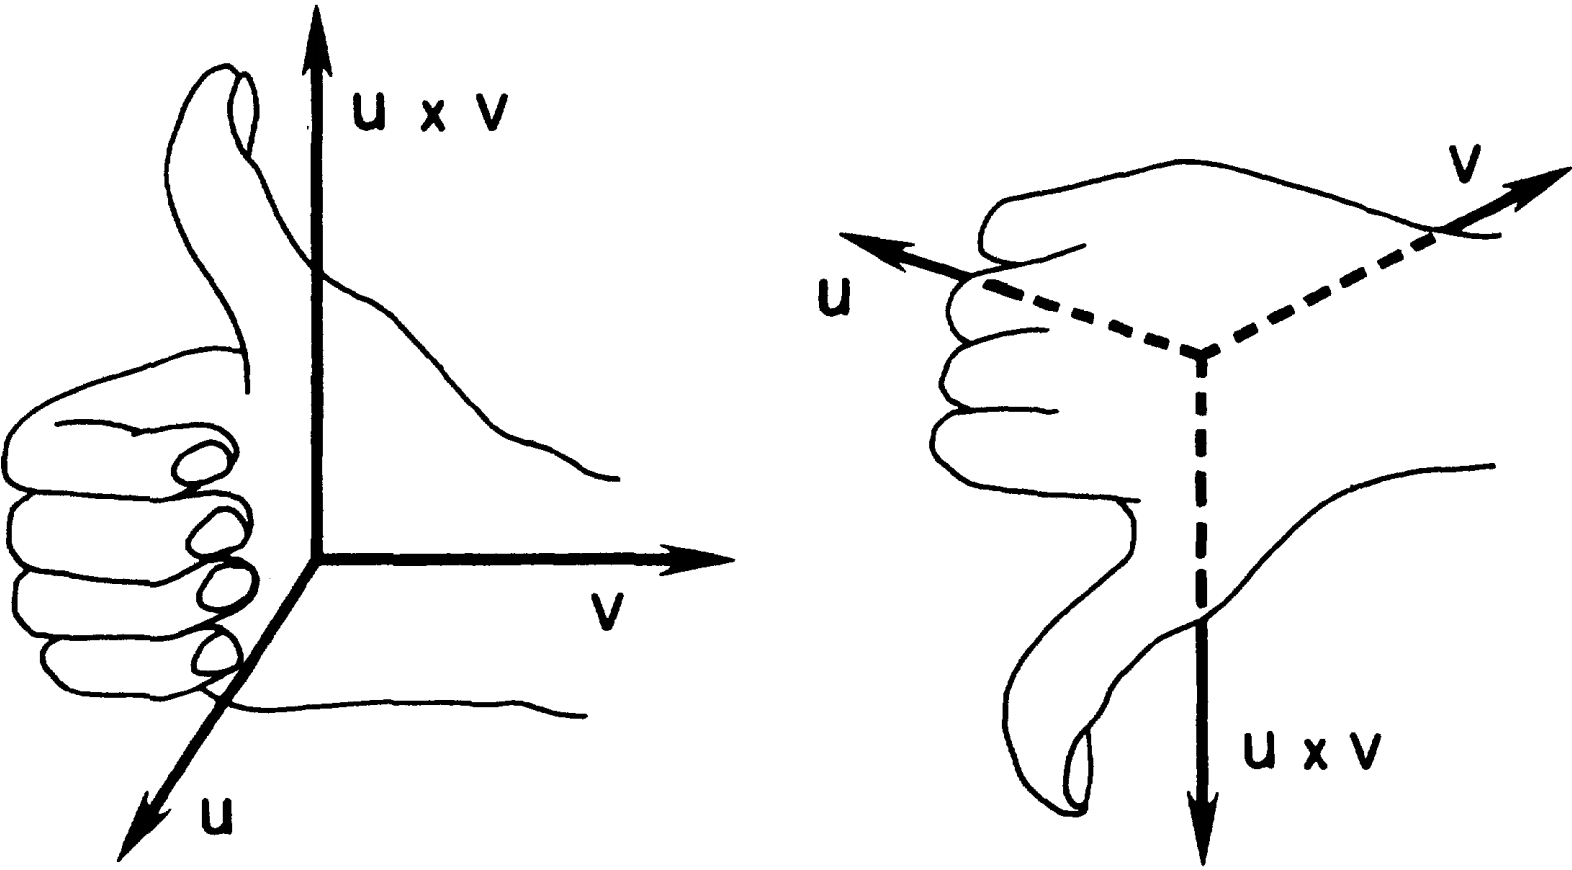
\includegraphics[width=0.85\textwidth]{./image/1.6.png}
        \caption{}
        \label{fig:1.6}
    \end{minipage}
    \begin{minipage}[b]{0.48\textwidth}
        \centering
        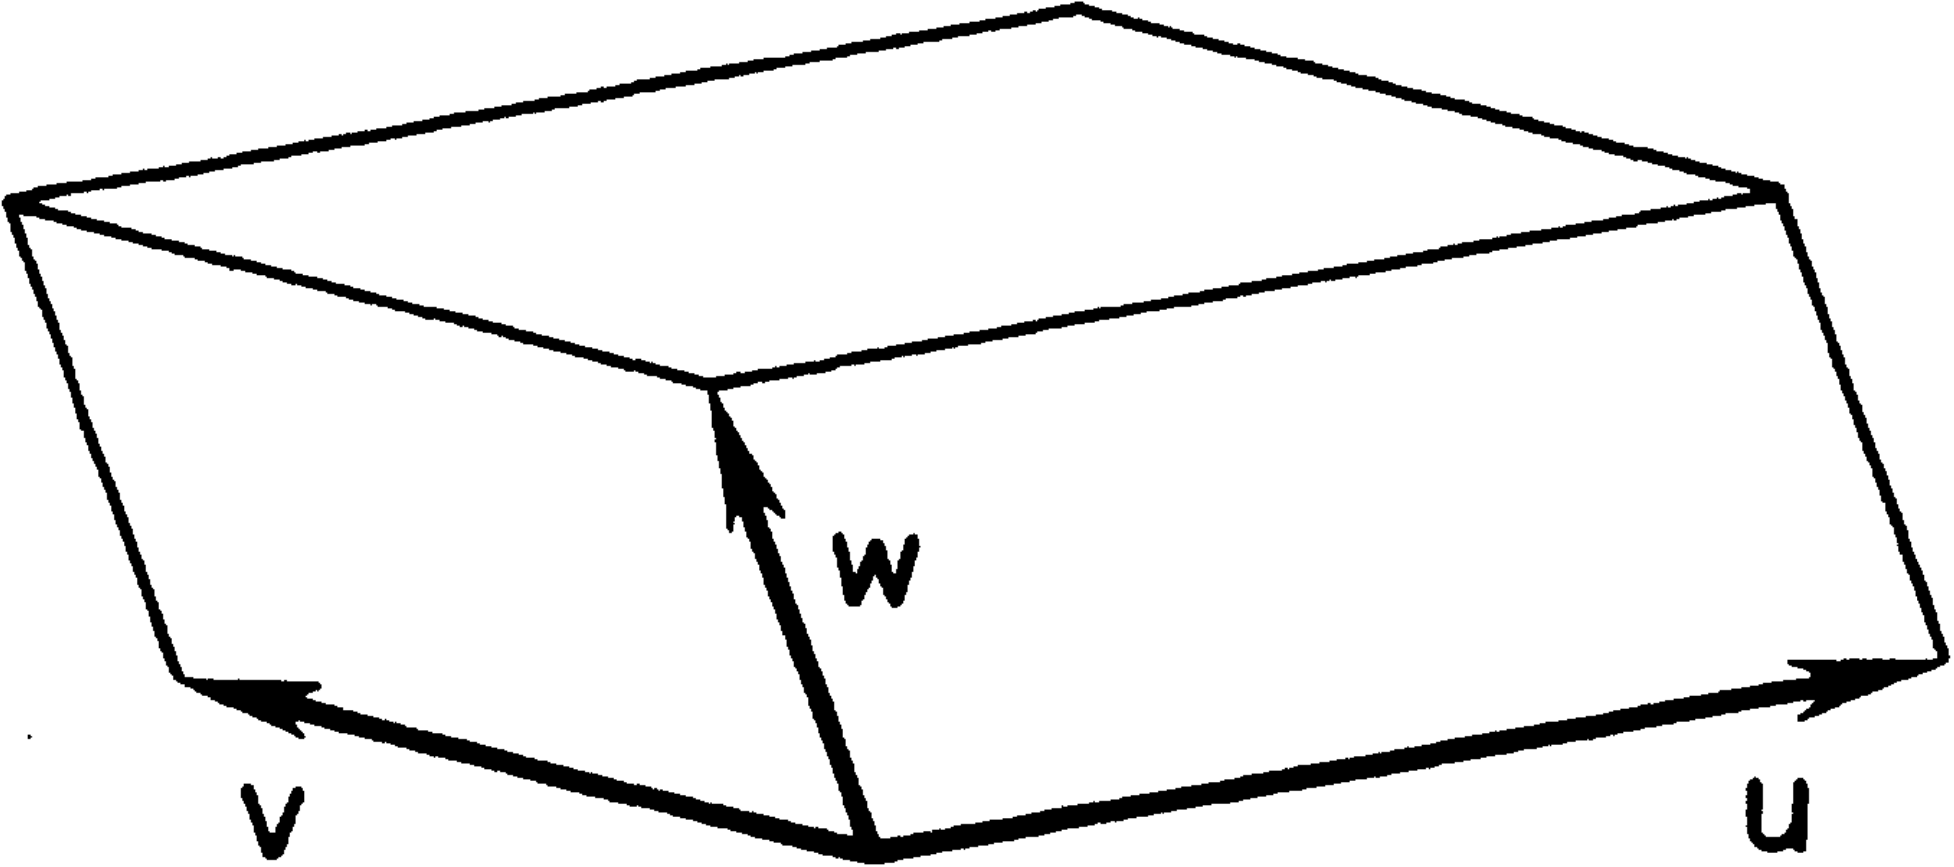
\includegraphics[width=0.85\textwidth]{./image/1.7.png}
        \caption{}
        \label{fig:1.7}
    \end{minipage}
\end{figure}

叉积进一步的用途在于三重混合积$(\bb{u}\times \bb{v})\cdot \bb{w}$的几何含义。考虑一个以$\bb{u}$、$\bb{v}$和$\bb{w}$作为共端边缘的平行六面体,将它的体积记作$\mathrm{vol}\left( \bb{u},\bb{v},\bb{w} \right) $。我们将平行六面体分割成一片片的片元,每一个片元的高度极小而底面都是$\bb{u}$和$\bb{v}$构成的平行四边形\footnote{几乎不需要微积分我们就给出这个模型。想象一副相同的牌,每一张都是平行四边形。纸牌组的体积是它的厚度乘以纸牌面的面积,如果纸牌组被剪切成平行六面体的形状,这个体积显然是没有变化的。(译者注:即祖逖原理。)},通过这样分割,我们有
\begin{equation}
    \mathrm{vol}\left( \bb{u},\bb{v},\bb{w} \right) =\left| \left( \bb{u}\times \bb{v} \right) \cdot \bb{w} \right|
\end{equation}
如果$(\bb{u},\bb{v},\bb{w})$以这样的顺序组成了一个右手系,如图\eqref{fig:1.7}所示,那么根据几何学我们可以得到
\begin{equation}\label{equ:1.20}
    \mathrm{vol}\left( \bb{u},\bb{v},\bb{w} \right) =\left( \bb{u}\times \bb{v} \right) \cdot \bb{w}=\left( \bb{v}\times \bb{w} \right) \cdot \bb{u}=\left( \bb{w}\times \bb{u} \right) \cdot \bb{v} \le 0
\end{equation}
换言之,$\left( \bb{u}\times \bb{v} \right) \cdot \bb{w}$具有轮换对称性。

借助式\eqref{equ:1.20}我们将证明:叉积服从加法分配律
\begin{equation}\label{equ:1.21}
    \bb{u}\times \left( \bb{v}+\bb{w} \right) =\bb{u}\times \bb{v}+\bb{u}\times \bb{w}
\end{equation}
为此,我们引入一个定理:两个矢量相等,当且仅当它们与任意一个矢量$\bb{c}$的点积相等\footnote{为什么?好吧,我们来证明:。首先,如果已知$\bb{u}=\bb{v}$,那么由此可推出,对于任意矢量$\bb{c}$,$\bb{u}\cdot \bb{c}=\bb{v}\cdot \bb{c}$都成立;反过来讲,若已知对于任意矢量$\bb{c}$,$\bb{u}\cdot \bb{c}=\bb{v}\cdot \bb{c}$都成立,我们可以设$\bb{c}=\bb{u}-\bb{v}$,此时有
\begin{align*}
	\bb{u}\cdot \bb{c}&=\bb{v}\cdot \bb{c}\\
	\bb{u}\cdot \bb{c}-\bb{v}\cdot \bb{c}&=0\\
	\left( \bb{u}-\bb{v} \right) \cdot \left( \bb{u}-\bb{v} \right) &=0\\
	\left| \bb{u}-\bb{v} \right|^2&=0
\end{align*}
可以导出$\bb{u}-\bb{v}=0$,也就是说,$\bb{u}=\bb{v}$。
}。由此

\begin{align*}
	\left[ \bb{u}\times \left( \bb{v}+\bb{w} \right) \right] \cdot \bb{c}&=\left( \bb{c}\times \bb{u} \right) \cdot \left( \bb{v}+\bb{w} \right)\\
	&=\left( \bb{c}\times \bb{u} \right) \cdot \bb{v}+\left( \bb{c}\times \bb{u} \right) \cdot \bb{w}\\
	&=\left( \bb{u}\times \bb{v} \right) \cdot \bb{c}+\left( \bb{u}\times \bb{w} \right) \cdot \bb{c}\\
	&=\left( \bb{u}\times \bb{v}+\bb{u}\times \bb{w} \right) \cdot \bb{c}
\end{align*}
\qed

\begin{example}
    不用分量,证明:三重矢积公式:
    \begin{equation}\label{equ:1.22}
        \left( \bb{u}\times \bb{v} \right) \times \bb{w}=\left( \bb{w}\cdot \bb{u} \right) \bb{v}-\left( \bb{w}\cdot \bb{v} \right) \bb{u}
    \end{equation}
\end{example}
\begin{solution}
    $\bb{u}\times \bb{v}$必然垂直于$\bb{u}$、$\bb{v}$所在平面。因此,$\left( \bb{u}\times \bb{v} \right) \times \bb{w}$必然垂直于$\left( \bb{u}\times \bb{v} \right) $、$\bb{w}$所在平面,躺在$\bb{u}$、$\bb{v}$所在平面上,因此我们设
    \begin{equation}\label{equ:Example 1.2*}
         \left( \bb{u}\times \bb{v} \right) \times \bb{w}=A\bb{u}+B\bb{v}\tag{*}
    \end{equation}
    其中,$A$、$B$为关于$\bb{u},\bb{v},\bb{w}$的未知标量函数。式\eqref{equ:Example 1.2*}的左边垂直于$\bb{w}$,因此可以得到
    \begin{equation*}
        0=A\bb{u}\cdot \bb{w}+B\bb{v}\cdot \bb{w}
    \end{equation*}
    我们设
    \begin{equation*}
        A=-C\left( \bb{v}\cdot \bb{w} \right) \,\, ,  B=C\left( \bb{u}\cdot \bb{w} \right) 
    \end{equation*}
    其中,$C$为关于$\bb{u},\bb{v},\bb{w}$的未知标量函数。因此
    \begin{equation}\label{equ:Example 1.2**}
         \left( \bb{u}\times \bb{v} \right) \times \bb{w}=C\left( \bb{u},\bb{v},\bb{w} \right) \left[ \left( \bb{u}\cdot \bb{w} \right) \bb{v}-\left( \bb{v}\cdot \bb{w} \right) \bb{u} \right] \tag{**}
    \end{equation}
    特别地,当$\bb{w}=\bb{u}$时,式\eqref{equ:Example 1.2**}简化为
    \begin{equation}\label{equ:Example 1.2***}
         \left( \bb{u}\times \bb{v} \right) \times \bb{u}=C\left( \bb{u},\bb{v},\bb{u} \right) \left[ \left| \bb{u} \right|^2\bb{v}-\left( \bb{v}\cdot \bb{u} \right) \bb{u} \right] \tag{$\begin{subarray}{c}
            *\\
            **
        \end{subarray}$}
    \end{equation}
    用$\bb{v}$点乘等式两边,并对左边进行整理,我们可以得到
    \begin{equation}\label{equ:Example 1.2****}
         \left( \bb{u}\times \bb{v} \right) \cdot \left( \bb{u}\times \bb{v} \right) =C\left( \bb{u},\bb{v},\bb{u} \right) \left[ \left| \bb{u} \right|^2\left| \bb{v} \right|^2-\left( \bb{u}\cdot \bb{v} \right) ^2 \right] \tag{$\begin{subarray}{c}
            **\\
            **
        \end{subarray}$}
    \end{equation}
    但是
    \begin{align*}
        \left( \bb{u}\times \bb{v} \right) \cdot \left( \bb{u}\times \bb{v} \right) &=\left| \bb{u}\times \bb{v} \right|^2\\
        &=\left| \bb{u} \right|^2\left| \bb{v} \right|^2\sin ^2\theta\\
        &=\left| \bb{u} \right|^2\left| \bb{v} \right|^2\left( 1-\cos ^2\theta \right)\\
        &=\left| \bb{u} \right|^2\left| \bb{v} \right|^2-\left( \bb{u}\cdot \bb{v} \right) ^2
    \end{align*}
    对比这个表达式的最后一行和式\eqref{equ:Example 1.2****}的右边,我们可以得到${ C\left( \bb{u},\bb{v},\bb{u} \right) =1}$。

    现在,用$\bb{u}$点乘式\eqref{equ:Example 1.2**}两边,整理左边的三重标积,我们有
    \begin{equation*}
        \left[ \bb{u}\times \left( \bb{u}\times \bb{v} \right) \right] \cdot \bb{w}=C\left( \bb{u},\bb{v},\bb{w} \right) \left[ \left( \bb{u}\cdot \bb{w} \right) \left( \bb{v}\cdot \bb{u} \right) -\left( \bb{v}\cdot \bb{w} \right) \left| \bb{u} \right|^2 \right] 
    \end{equation*}
    但是我们在上述讨论中得出了式\eqref{equ:Example 1.2***}中${ C\left( \bb{u},\bb{v},\bb{u} \right) =1}$,因此有
    \begin{equation*}
        \left[ \left( \bb{u}\times \bb{v} \right) \times \bb{w} \right] \cdot \bb{u}=\left( \bb{u}\cdot \bb{w} \right) \left( \bb{v}\cdot \bb{u} \right) -\left( \bb{v}\cdot \bb{w} \right) \left| \bb{u} \right|^2
    \end{equation*}

    因此${ C\left( \bb{u},\bb{v},\bb{w} \right) =1}$

    \qed
\end{solution}
在投影面积方面,三重标积有另一种实用的解释。见习题1.15。

我们如何找到$\bb{u}\times \bb{v}$的笛卡尔坐标?这不像 $\bb{u}\cdot \bb{v}$那么简单。一方面是因为,$\bb{u}\times \bb{v}$是矢量而不是标量,而另一方面,$\bb{u}\times \bb{v}$是一只生活在三维空间中的野兽!(Grassmann 创建了一个代数体系,它为高维欧几里德空间中诸如$\bb{u}\times \bb{v}$或$\bb{u}\times \bb{v}\times \bb{w}$之类的对象赋予了意义,在这些空间中,它们被称为楔积。)一种直接(但乏味)的方法是重复应用分配律\eqref{equ:1.21},我们置
\begin{align}
	\bb{u}\times \bb{v}&=\left( u_x\bf{e}_x+u_y\bf{e}_y+u_z\bf{e}_z \right) \times \left( v_x\bf{e}_x+v_y\bf{e}_y+v_z\bf{e}_z \right)\nonumber\\
	&=u_xv_x\bf{e}_x\times \bf{e}_x+u_xv_y\bf{e}_x\times \bf{e}_y+u_xv_z\bf{e}_x\times \bf{e}_z\nonumber\\
	&+u_yv_x\bf{e}_y\times \bf{e}_x+u_yv_y\bf{e}_y\times \bf{e}_y+u_yv_z\bf{e}_y\times \bf{e}_z\nonumber\\
	&+u_zv_x\bf{e}_z\times \bf{e}_x+u_zv_y\bf{e}_z\times \bf{e}_y+u_zv_z\bf{e}_z\times \bf{e}_z\label{equ:1.23}
\end{align}
(烦死啦!)但是,$\bf{e}_x\times \bf{e}_x=0,\bf{e}_x\times \bf{e}_y=\bf{e}_z,\bf{e}_x\times \bf{e}_z=-\bf{e}_y$……(画个图去!)因此式\eqref{equ:1.23}简化成
\begin{equation}\label{equ:1.24}
    \bb{u}\times \bb{v}=\bf{e}_x\left( u_yv_z-u_zv_y \right) +\bf{e}_y\left( u_zv_x-u_xv_z \right) +\bf{e}_z\left( u_xv_y-u_yv_x \right) 
\end{equation}
式\eqref{equ:1.24}一种简单的记忆方法是将它写成
\begin{equation}\label{equ:1.25}
    \bb{u}\times \bb{v}=\left| \begin{matrix}
        \bf{e}_x&		\bf{e}_y&		\bf{e}_z\\
        u_x&		u_y&		u_z\\
        v_x&		v_y&		v_z\\
    \end{matrix} \right|
\end{equation}
其中,行列式应围绕第一行展开。

从式\eqref{equ:1.24}、式\eqref{equ:1.25}和行列式的性质,即行列转置值不变,交换两行(或列)改变符号,我们得到有用的公式
\begin{equation}\label{equ:1.26}
    (\bb{u}\times \bb{v})\cdot \bb{w}=\left| \begin{matrix}
        w_x&		w_y&		w_z\\
        u_x&		u_y&		u_z\\
        v_x&		v_y&		v_z\\
    \end{matrix} \right|=\left| \begin{matrix}
        u_x&		u_y&		u_z\\
        v_x&		v_y&		v_z\\
        w_x&		w_y&		w_z\\
    \end{matrix} \right|=\left| \begin{matrix}
        u_x&		v_x&		w_x\\
        u_y&		v_y&		w_y\\
        u_z&		v_z&		w_z\\
    \end{matrix} \right|
\end{equation}

\begin{example}
    用两种方法(用叉积和不用叉积)给出一个单位矢量$\bf{e}$同时垂直于$\bb{a}\sim \left( 1,-2,3 \right) $和$\bb{b}\sim \left( -1,0,1 \right) $。
\end{example}
\begin{solution}
    如果用叉积的方法,我们寻找的矢量是
    \begin{equation*}
        \bf{e}=\pm \frac{\bb{a}\times \bb{b}}{\left| \bb{a}\times \bb{b} \right|}
    \end{equation*}
    根据式\eqref{equ:1.25}
    \begin{equation*}
        \bb{a}\times \bb{b}=\left| \begin{matrix}
            \bf{e}_x&		\bf{e}_y&		\bf{e}_z\\
            1&		-2&		3\\
            -1&		0&		1\\
        \end{matrix} \right|\sim \left( -2,-4,-2 \right) 
    \end{equation*}
    因为$\left| \bb{a}\times \bb{b} \right|=2\sqrt{6}$,因此$\bf{e}\sim \pm \left( 1/\sqrt{6},2/\sqrt{6},1/\sqrt{6} \right) $

    不用叉积的方法计算$\bf{e}$,我们可以设$\bf{e}\sim \left( a,b,c \right) $。那么我们可以得到
    \begin{equation*}
        \left\{ \begin{aligned}
            \bf{e}\cdot \bb{a}&=a-2b+3c=0\\
            \bf{e}\cdot \bb{b}&=-a+c=0\\
        \end{aligned} \right. 
    \end{equation*}
    为了使$\left| \bf{e} \right|=1$,我们可以取$a=\pm 1/\sqrt{6}$,代入即可。
\end{solution}

